%******************************************************************************
% KOMA-Script article scrartcl
%******************************************************************************
\documentclass[12pt, b5paper]{article} 

% Add here all the packages that will be used in the document
%******************************************************************************
% Packages 
%******************************************************************************
% For hyperlinks 
\usepackage{url}

% Add no chapters to the article 
\usepackage[nochapters]{classicthesis}

% Setup the page geometry
\usepackage{geometry}
\geometry{a4paper, total={210mm, 297mm}, 
left=20mm, right=20mm, top=20mm, bottom=20mm}

% Use tikz to add watermarks to the document
\usepackage{blindtext,tikz}
\usetikzlibrary{calc}

% Use the classicthesis style for the style of the document
\usepackage[nochapters]{classicthesis} 

% Use the currvita style for the layout of the document
\usepackage[LabelsAligned]{currvita} 

% Required for adding links	and customizing them
\usepackage{hyperref} 

 % Set link colors
\hypersetup{colorlinks, breaklinks, urlcolor=Maroon, linkcolor=Maroon}


% Add a list of new commands 
%******************************************************************************
% Commands 
%******************************************************************************
\newcommand{\latex}{\LaTeX\xspace}
\newcommand{\tex}{\TeX\xspace}

\usepackage{listings}
\usepackage{color}
\usepackage{graphicx}
\usepackage{caption}
\usepackage{subcaption}

\graphicspath{{images/report6/}}

\definecolor{dkgreen}{rgb}{0,0.6,0}
\definecolor{gray}{rgb}{0.5,0.5,0.5}
\definecolor{mauve}{rgb}{0.58,0,0.82}

\lstset{frame=tb,
  language=Java,
  aboveskip=3mm,
  belowskip=3mm,
  showstringspaces=false,
  columns=flexible,
  basicstyle={\small\ttfamily},
  numbers=none,
  numberstyle=\tiny\color{gray},
  keywordstyle=\color{blue},
  commentstyle=\color{dkgreen},
  stringstyle=\color{mauve},
  breaklines=true,
  breakatwhitespace=true,
  tabsize=3
}

%******************************************************************************
% DOCUMENT STARTS HERE 
%******************************************************************************
\begin{document}

% TITLE 
\title{\rmfamily\normalfont\spacedallcaps{
Report \#{6}
}}

% PROJECT NAME -> ADD YOUR PROJECT NAME HERE
\author{{\small Automatic Mandible Segmentation Using VTK}}

% AUTOMATIC DATE -> DON'T CHANGE MANUALLY
\date{\footnotesize{\today}}

% MAKE THE TITLE -> DON'T CHANGE MANUALLY
\maketitle

% DON'T INCLUDE THE ABSTRACT FOR THE MOMENT
% % \begin{abstract}
% \noindent Abstract
% \end{abstract}
 
%******************************************************************************
% TABLE OF CONTENTS (uncomment to show / comment to hide)
%******************************************************************************     
% \tableofcontents


%******************************************************************************
% Report Content
%******************************************************************************
\section{Report Details}
\begin{center}
\begin{tabular}{ l | c }
\hline 
Report ID & 6  \\ % Change the sprint ID here 
\hline 
Report Duration & 1 Week \\ % Change the duration here 
\hline 
Beginning & 29.11.2016 \\ % Change the start data here
\hline 
End & 5.12.2016 \\ % Change the end data here
\hline 
\end{tabular}
\end{center}

%\section{Objectives}
\section{Original Objectives}
\begin{itemize}
\item Enabling GUI Support in VTK.
\item GUI Design.
\item Maxilla segmentation.
\item Teeth Segmentation.
\item X-Ray Effect.
\end{itemize}

\section{Accomplished Objectives}
\subsection{Enabling GUI Support in VTK}
To Enable GUI support of VTK Library I had to recompile the source code of the VTK library, and reconfigure CMake to generate a new Makefile and then I can compile the project and install it and use Qt wrapper classes to be able to design a GUI Application using Qt. It is mainly the \textit{QVTKWidget} class. But after I did that I found that it is not working as It by default compiled to support Qt4 not Qt5 that led me to recompile the VTK library again to make it supports Qt5 not Qt4 and finally it works.

\subsection{GUI Design}
After Enabling GUI Support in VTK library, I have designed an Initial GUI to be able to load any volume and set the segmentation parameters dynamically according to the used dataset, figure \ref{fig:GUI} shows the initial GUI taps I have a tap to load data and set the rendering mode and another tab to set segmentation paramters. As shown in figure \ref{fig:EX} I have loaded a sample dataset and I can using a slider set the iso value of the extracted surfaces interactively. I know that it is a poor GUI yet now but I will work to improve it and make it more functional and more interactive.
\begin{figure}
    \centering
    \begin{subfigure}[b]{0.65\textwidth}
        \centering
        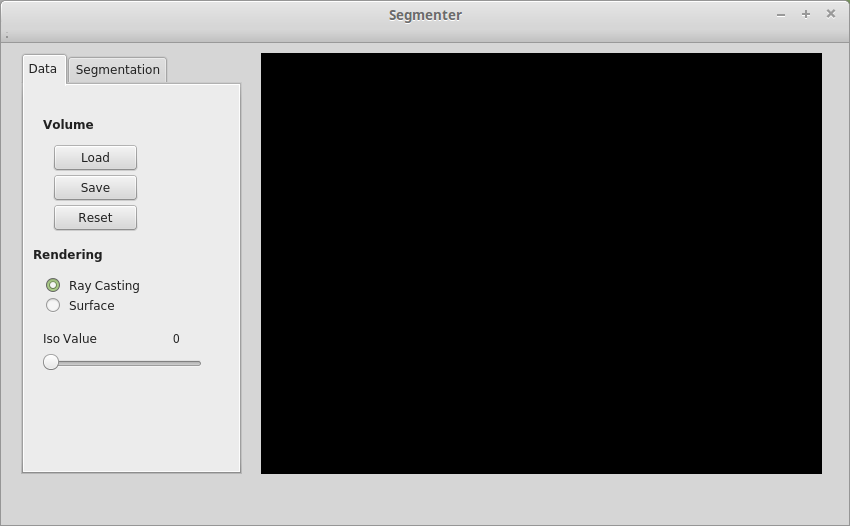
\includegraphics[width=\textwidth]{T1}
        \caption{Inital GUI Tap1}
    \end{subfigure}
    \hfill
    \begin{subfigure}[b]{0.65\textwidth}
        \centering
        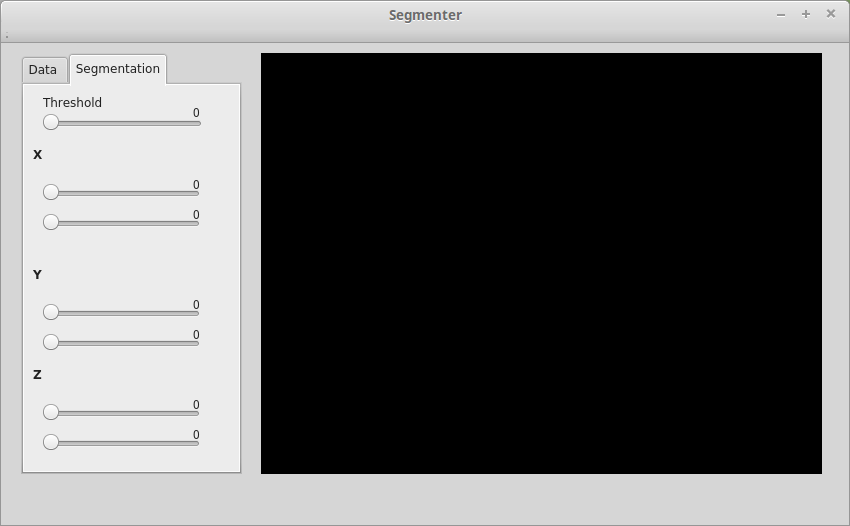
\includegraphics[width=\textwidth]{T2}
        \caption{Inital GUI Tap2}
    \end{subfigure}
    \caption{Initial GUI Design for Segmenter Application.}
    \label{fig:GUI}
\end{figure}


\begin{figure}
    \centering
    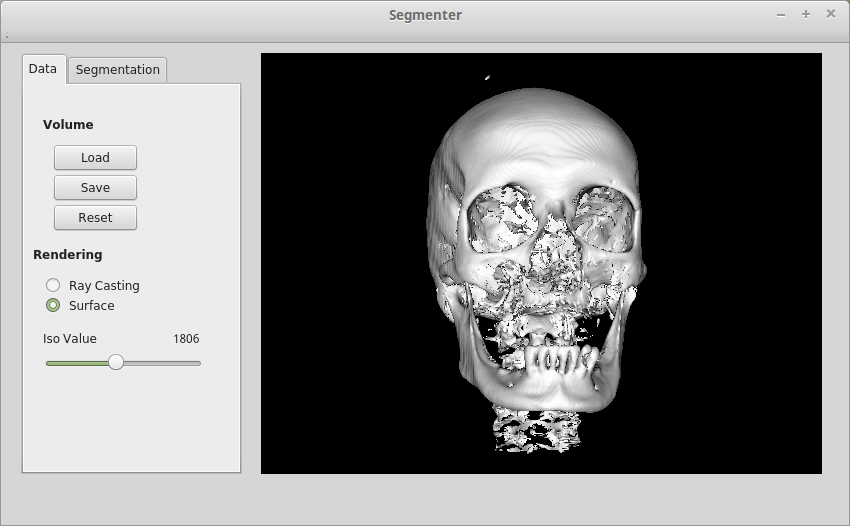
\includegraphics[scale=0.5]{EX}
    \caption{Rendering Example using Initial GUI}
    \label{fig:EX}
\end{figure}

\section{Missed Objectives}
\begin{itemize}
\item Maxilla segmentation.
\item Teeth Segmentation.
\item X-Ray Effect.
\end{itemize}

\section{Next Step}
\begin{itemize}
\item Enhance the GUI. 
\item Do missed objectives.
\end{itemize}
%******************************************************************************
% DOCUMENT ENDS HERE 
%******************************************************************************
\end{document}